
% The motivation behind EPG comes from the fact that propagating the by using a compact basis set of $\bm{F_k}$ and $\bm{Z_{k}}$ coefficients to represent the huge collection of spins that can be found in a voxel, 
% --- If we assume gradient areas are quantized into units that give a phase twist  of one cycle ($2\pi$) across a voxel then we can easily represent large groups of spins with a simple fourier basis, and accurately calculate MR signals

% \hfill
% 
% Mathematically, these configuration states are related to
% %form a Fourier pair with 
% the complex transverse magnetisation $M_{+}$ and longitudinal magnetisation $M_z$ \cite{Hennig1991} through:
% \begin{equation}
% \begin{split}
%     F_{k}  & = \int_0^1 M_{+}(z) e^{- i 2\pi k z} dz \\ %& \Longleftrightarrow M_{+}(z) = \int_{- \infty}^{+ \infty}  F_{k} e^{+ i 2\pi k z} dk \\
%     F_{-k} & = \int_0^1 M_{-}(z) e^{- i 2\pi k z} dz \\ %& \Longleftrightarrow M_{-}(z) = \int_{- \infty}^{+ \infty}  F_{-k} e^{+ i 2\pi k z} dk \\
%     Z_{k} & = \int_0^1 M_{z}(z) e^{- i 2\pi k z} dz %& \Longleftrightarrow M_{z}(z) = \int_{- \infty}^{+ \infty} Z_{k} e^{+ i 2\pi k z} dk
% \end{split}    
% \end{equation}
% where z is the voxel dimension and is in the $[0,1]$ range (without loss of generality) and $M_+ = (M_-)^*$.
% The $F_{k}$ and $F_{-k}$ states can be thought of as a two counter-rotating isochromat populations \cite{Brown}.

\hfill

\textbf{The $\bm{F_0}$ and $\bm{Z_0}$ configuration states}

% In this section we explain the main ingredients behind the EPG formalism, starting from a simple example of a fully relaxed spin system.
%In order to model the behaviour of a spin ensemble with known relaxation times and proton density values in a single-voxel MRF-\ac{fisp} sequence, 
%In order to simulate the magnetisation dynamics in this multi-pulse sequence, 
%we begin with the description of a single $T_R$ block.
%In order to 
% To simplify things even further, we begin with the thermal equilibrium case, where the spin ensemble is fully relaxed and the magnetic moment vectors have the same direction as the main magnetic field (here considered to be $\hat{z}$).
At thermal equilibrium, an isochromat ensemble is fully relaxed and the magnetic moment vectors have the same direction as the main magnetic field (here considered to be $\hat{z}$).
This state in which the spin system is initially found is called a $\bm{Z_0}$ configuration \cite{Weigel2015} \cite{Scheffler1999} \cite{Hennig1991}.
The coefficient for this state is equal to $1$ as the entire population of the imaginary spin ensemble is found in this configuration.
Pictorially, the $\bm{Z_0}$ state is shown in Figure~\ref{fig:Z0F0states} a) where I chose to represent 100 uniformly distributed isochromats along the voxel dimension.

\hfill

The application of an instantaneous $\pi/2$ excitation pulse on this configuration has the effect of `flipping' the entire isochromat ensemble in the transverse plane.
This new configuration is known as the $\bm{F_0}$ state \cite{Weigel2015} \cite{Scheffler1999} \cite{Hennig1991} (with a coefficient equal to $1$) and is graphically shown in Figure~\ref{fig:Z0F0states} b).
The $\bm{F_0}$ configuration is an important concept in the \ac{epg} formalism as it represents coherent transverse magnetisation and it is the cause of echo generation.

% 
% \hfill
% 
% The isochromat ensemble can `flip' back and forth between the two states by the application of the same instantaneous $\pi/2$ pulse.

\begin{figure}[ht]
    \centering
    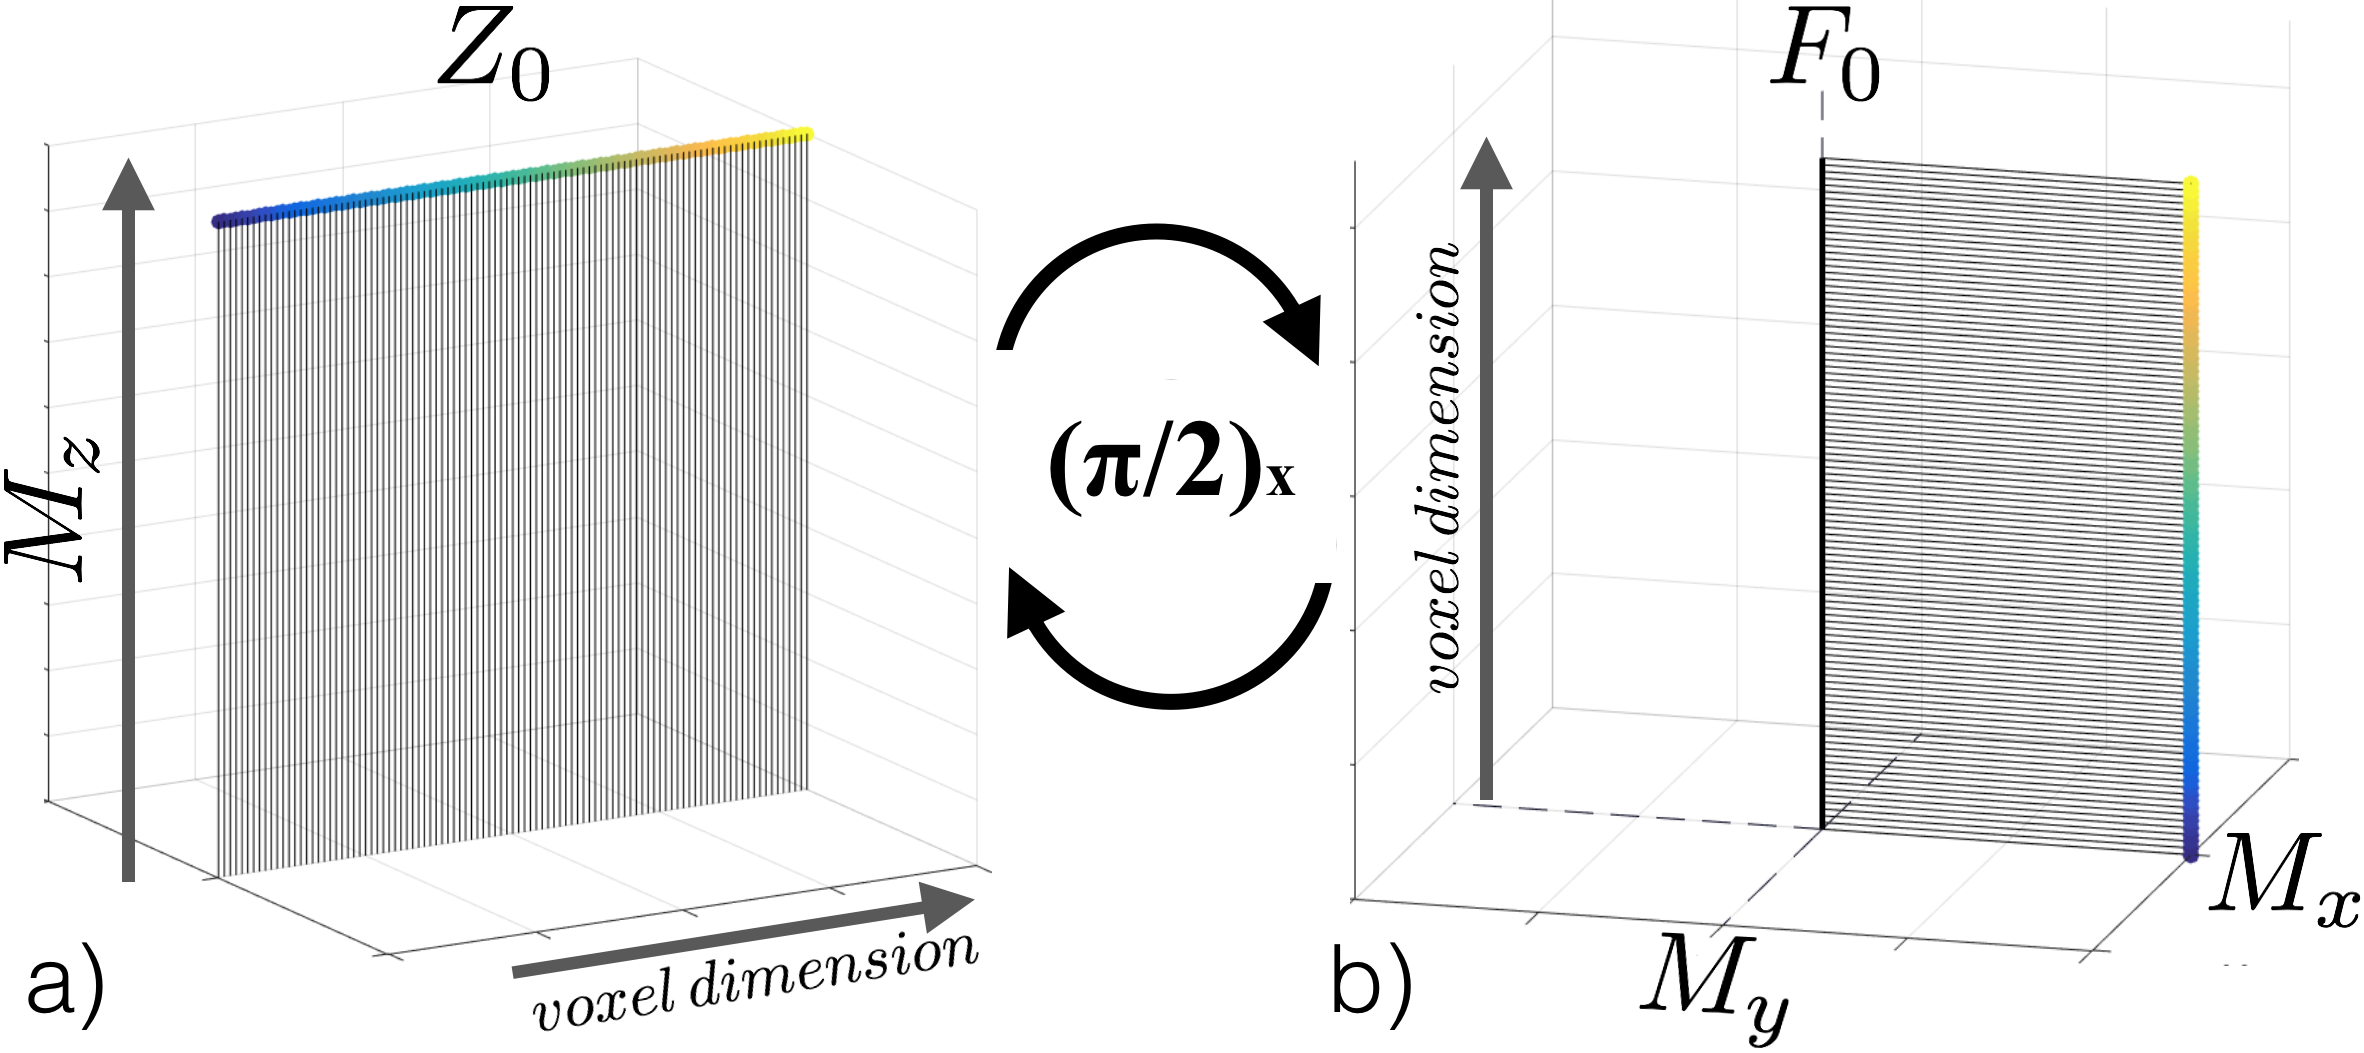
\includegraphics[angle=0,width=0.65\textwidth, keepaspectratio]{images/mrf/Z0F0states}
    \caption{The figure shows a pictorial representation of a single 1D voxel with uniform density of magnetisation.
    a) $\bm{Z_0}$ is a configuration in which the isochromat ensemble is characterised by spins lying along $M_z$.
    b) $\bm{F_0}$ is a configuration in which the isochromat ensemble is characterised by coherent transverse magnetisation.
    An instantaneous $\pi/2$ excitation pulse can `flip' the isochromat ensemble back and forth between the two states.
    It is important to note that a $(\pi/2)_x$ RF pulse applied on the $\bm{F_0}$ state will cause the isochromat ensemble to be pointing in the $- \hat{z}$ direction instead of the $+ \hat{z}$ direction it was initially found.
    However, this is still considered a $\bm{Z_0}$ configuration.
    }
    \label{fig:Z0F0states}
\end{figure}

% The formation of both $k = 0$ and $k \neq 0$ configuration states is a consequence of applying gradients and RF pulses.
% In particular, gradients induce phase twists in the isochromat ensemble, while RF pulses mix coefficients between states of equal $k$ values.
% In the following section the magnetisation dynamics in the FISP multi-pulse sequence is explained, starting with a single repetition period block and ending with the dictionary generation.

% % % % % % % % % % % % % % % % % % % % 
\textbf{The effect of a constant gradient on the isochromat ensemble} 

The application of a constant gradient introduces a linearly position-dependent off-resonance Larmor frequency on the isochromat ensemble along its axis (which is the same as the voxel dimension, as stated in the assumptions).
This can be seen in Figure~\ref{fig:effectOfGradsEPG} where after the first application of the gradient the spin system is now dephased.
This dephased configuration can be conceptually represented as an evenly distributed collection of magnetisation vectors called $\bm{F_1}$ \cite{Hennig1988} \cite{Scheffler1999}, where $\bm{k=1}$ represents one cycle of phase.
% Let us now introduce a dephasing gradient in the $\hat{z}$ direction (the 1D voxel's direction) that obeys the assumptions we previously described.
% This gradient induces phase accrual on the isochromat ensemble such that the isochromat found at one edge of the voxel is positioned at the `isocentre', while the isochromat found at the opposite edge experiences $2\pi$ dephasing.
% In fact, the off-resonance frequency increases linearly with the distance from the assumed `isocentre'.

\hfill

Each further application of the gradient increases the amount of dephasing experienced by the spin system with multiples of $2\pi$.
This can be seen in Figure~\ref{fig:effectOfGradsEPG} where each new application of the gradient `shifts' the spin system into a different configuration state.
These dephased configuration states are called $\bm{F_k}$, where $k$ represents the amount of $2\pi$ dephasing experienced by the spin ensemble.

% % % dephased magnetisation
\begin{figure}[H]
    \centering
    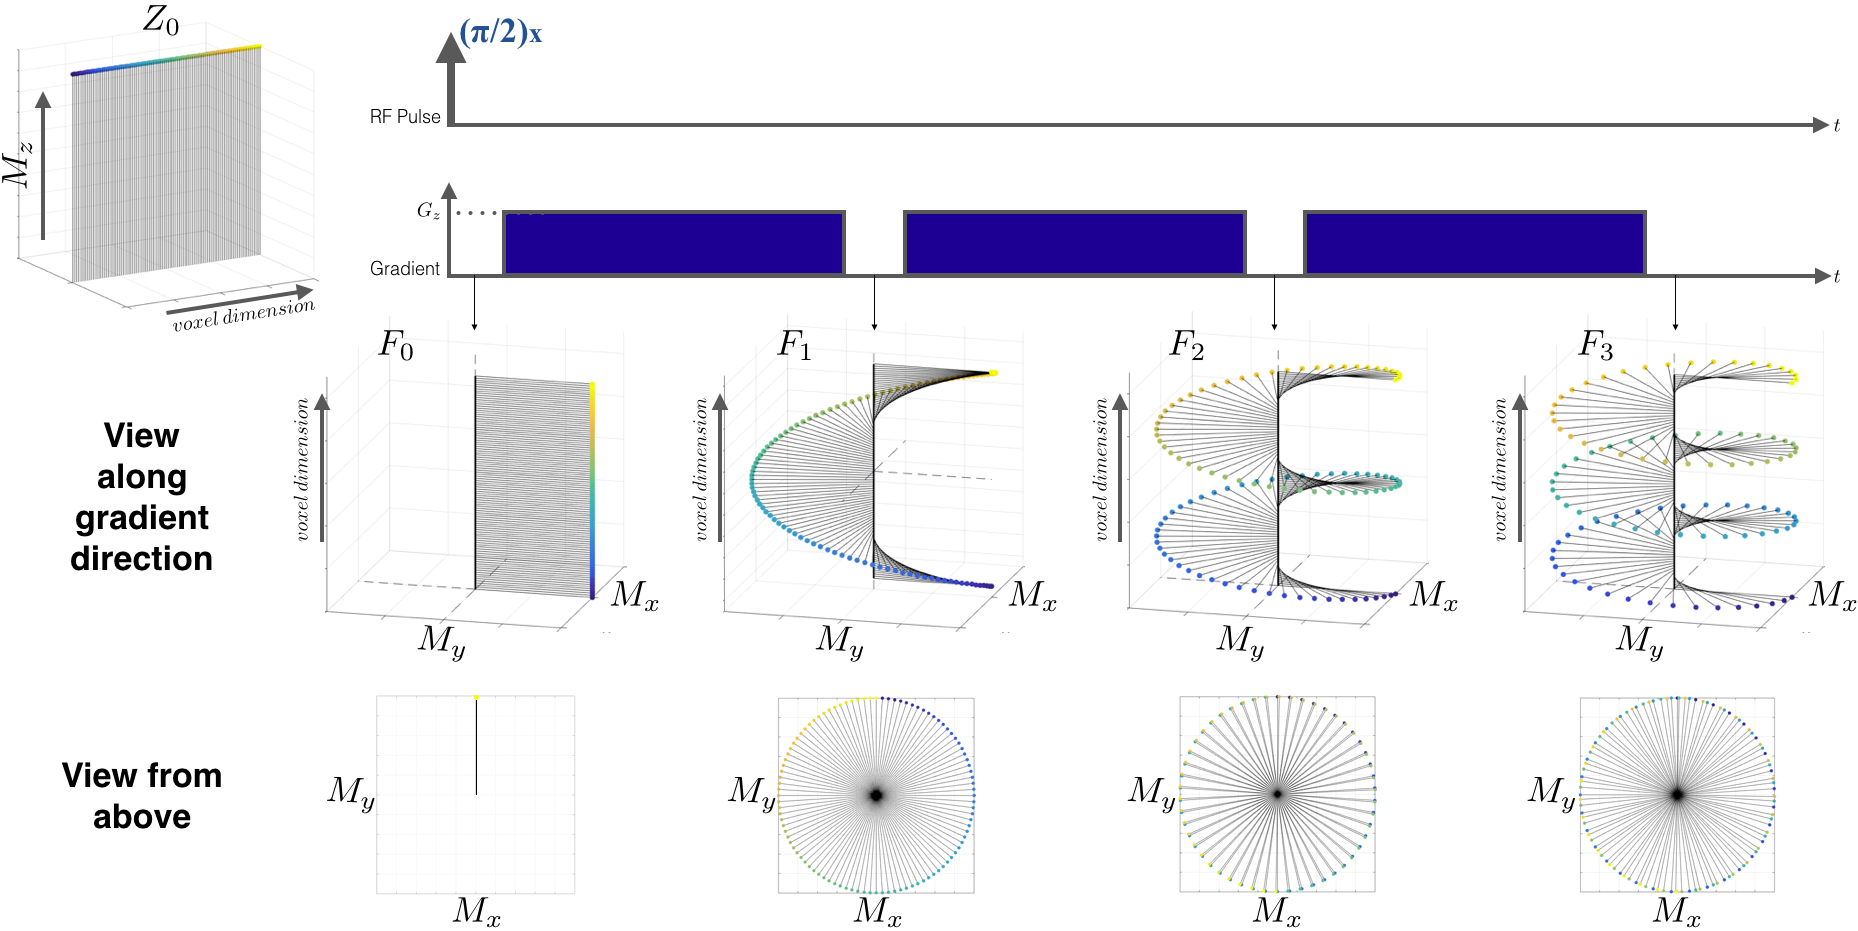
\includegraphics[angle=90,width=0.7\textwidth, keepaspectratio]{images/mrf/effectOfGradsEPG}
    \caption{Pictorial representation of an isochromat ensemble experiencing an ideal instantaneous $(\pi/2)_x$ RF pulse and dephasing induced by a gradient.
    This spin system is found in a 1D voxel whose dimension in along the same direction as the applied gradient (here, the $\hat{z}$ direction is considered) and which is positioned such that one edge of the voxel is at the `isocentre'. The isochromats found at the opposite edge accrue a phase of $2\pi$ after the application of this gradient.
    Every time the gradient is applied the spin system dephases further into a new configuration here represented as discrete states: $\bm{F_k}$.}
    \label{fig:effectOfGradsEPG}
\end{figure}

% % % % % % % % % % % % % % % % % % % % 
\textbf{The effect of an RF pulse on the isochromat ensemble} 

The application of an RF pulse of arbitrary flip angle $\alpha$ and phase angle $\phi$ on a dephased isochromat ensemble mixes the populations of spins among configurations.
This effect is best explained through equation \ref{eq:rfpulseequationbssfp}, which says that the magnetisation vectors immediately after the RF pulse are related to those immediately before the RF pulse through a rotation matrix (relaxation effects are neglected as the RF pulse is assumed to be instantaneous).
For completion, I rewrite equation \ref{eq:rfpulseequationbssfp} here:

\begin{equation}
    \begin{bmatrix} 
    M_x \\
    M_y \\
    M_z
    \end{bmatrix}^+ = 
        R_{\phi}(\alpha)
    \begin{bmatrix} 
    M_x \\
    M_y \\
    M_z
    \end{bmatrix}^-
\end{equation}
where, as before, superscript $+$ denotes `immediately after RF pulse' and superscript $-$ denotes 'immediately before RF pulse'.

\hfill

In complex notation, where $M_+ \equiv M_x + i M_y$,  $M_- \equiv M_x - i M_y$ and $M_- = (M_+)^*$ this becomes:

\begin{equation}\label{eq:magnbeforestates}
    \begin{bmatrix} 
    M_+ \\
    M_- \\
    M_z
    \end{bmatrix}^+ = 
        T_{\phi}(\alpha)
    \begin{bmatrix} 
    M_+ \\
    M_- \\
    M_z
    \end{bmatrix}^-
\end{equation}
where 
\begin{equation}\label{eq:woessnerFn2}
    T_{\phi}(\alpha) = 
    \begin{bmatrix}
        cos^2(\alpha/2) & e^{2i\phi} sin^2(\alpha/2) & - i e^{i \phi} sin(\alpha) \\
        e^{-2i\phi} sin^2(\alpha/2) & cos^2(\alpha/2) & i e^{-i \phi} sin(\alpha) \\
        - i/2 e^{-i \phi} sin(\alpha) & i/2 e^{i \phi} sin(\alpha) & cos \alpha
    \end{bmatrix}
\end{equation}

\hfill

% A completely dephased isochromat ensemble is rotated through an angle by the applied instantaneous RF pulse.
% This is seen in Figure~\ref{fig:RFpulseeffect} where we chose $\phi = 0$.

% \begin{figure}[ht]
%     \centering
%     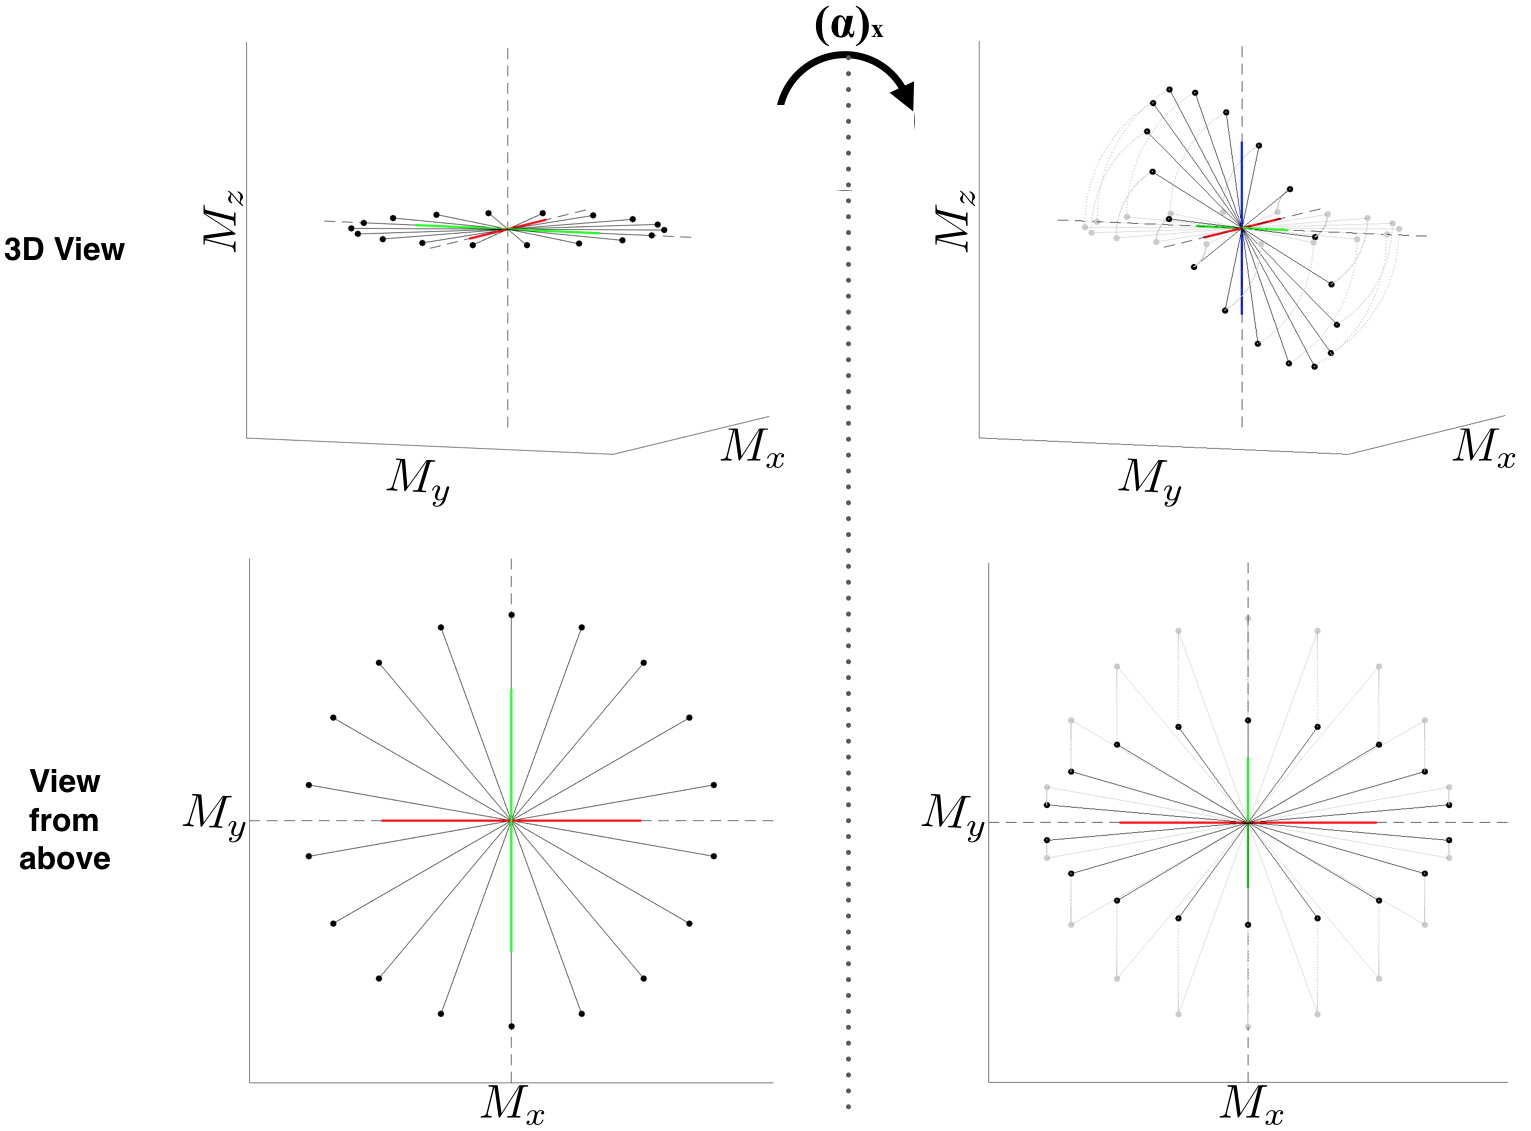
\includegraphics[angle=0,width=1\textwidth, keepaspectratio]{images/mrf/RFpulseeffect}
%     \caption{Pictorial representation of a completely dephased isochromat ensemble experiencing an ideal instantaneous $(\alpha)_x$ RF pulse.}
%     \label{fig:RFpulseeffect}
% \end{figure}
The transition to configuration states is straight forward, as the complex magnetisation vectors can be easily replaced with the partition states (the details of which are found in Hennig \cite{Hennig1991}).
Equation \ref{eq:magnbeforestates} becomes:

\begin{equation}\label{eq:magnafterstates}
    \begin{bmatrix} 
    F_{k} \\
    F_{-k} \\
    Z_{k}
    \end{bmatrix}^+ = 
        T_{\phi}(\alpha)
    \begin{bmatrix} 
    F_{k} \\
    F_{-k} \\
    Z_{k}
    \end{bmatrix}^-
\end{equation}

\hfill 

Expanding equation \ref{eq:magnafterstates} into its components yields:
\begin{equation}\label{eq:woessner}
\begin{split}
    F_{k}^+ &= F_{k}^- cos^2(\alpha/2) + e^{2i\phi} F_{-k}^- sin^2(\alpha/2)  - i e^{i \phi} Z_{k}^- sin(\alpha)  \\
    F_{-k}^+ &=  e^{-2i\phi} F_{k}^- sin^2(\alpha/2) + F_{-k}^- cos^2(\alpha/2) + i e^{-i \phi} Z_{k}^- sin(\alpha) \\
    Z_{k}^+ &= - i/2 e^{-i \phi} F_{k}^- sin(\alpha) + i/2 e^{-i \phi} F_{-k}^- sin(\alpha) + Z_{k}^- cos(\alpha) 
\end{split}
\end{equation}
which is known as the \textbf{Woessner decomposition} and it shows that in the case of an arbitrary RF pulse, the population of isochromats is redistributed among states with the same amount of dephasing $k$ \cite{Hennig1991}.

\hfill

\begin{figure}[H]
    \centering
    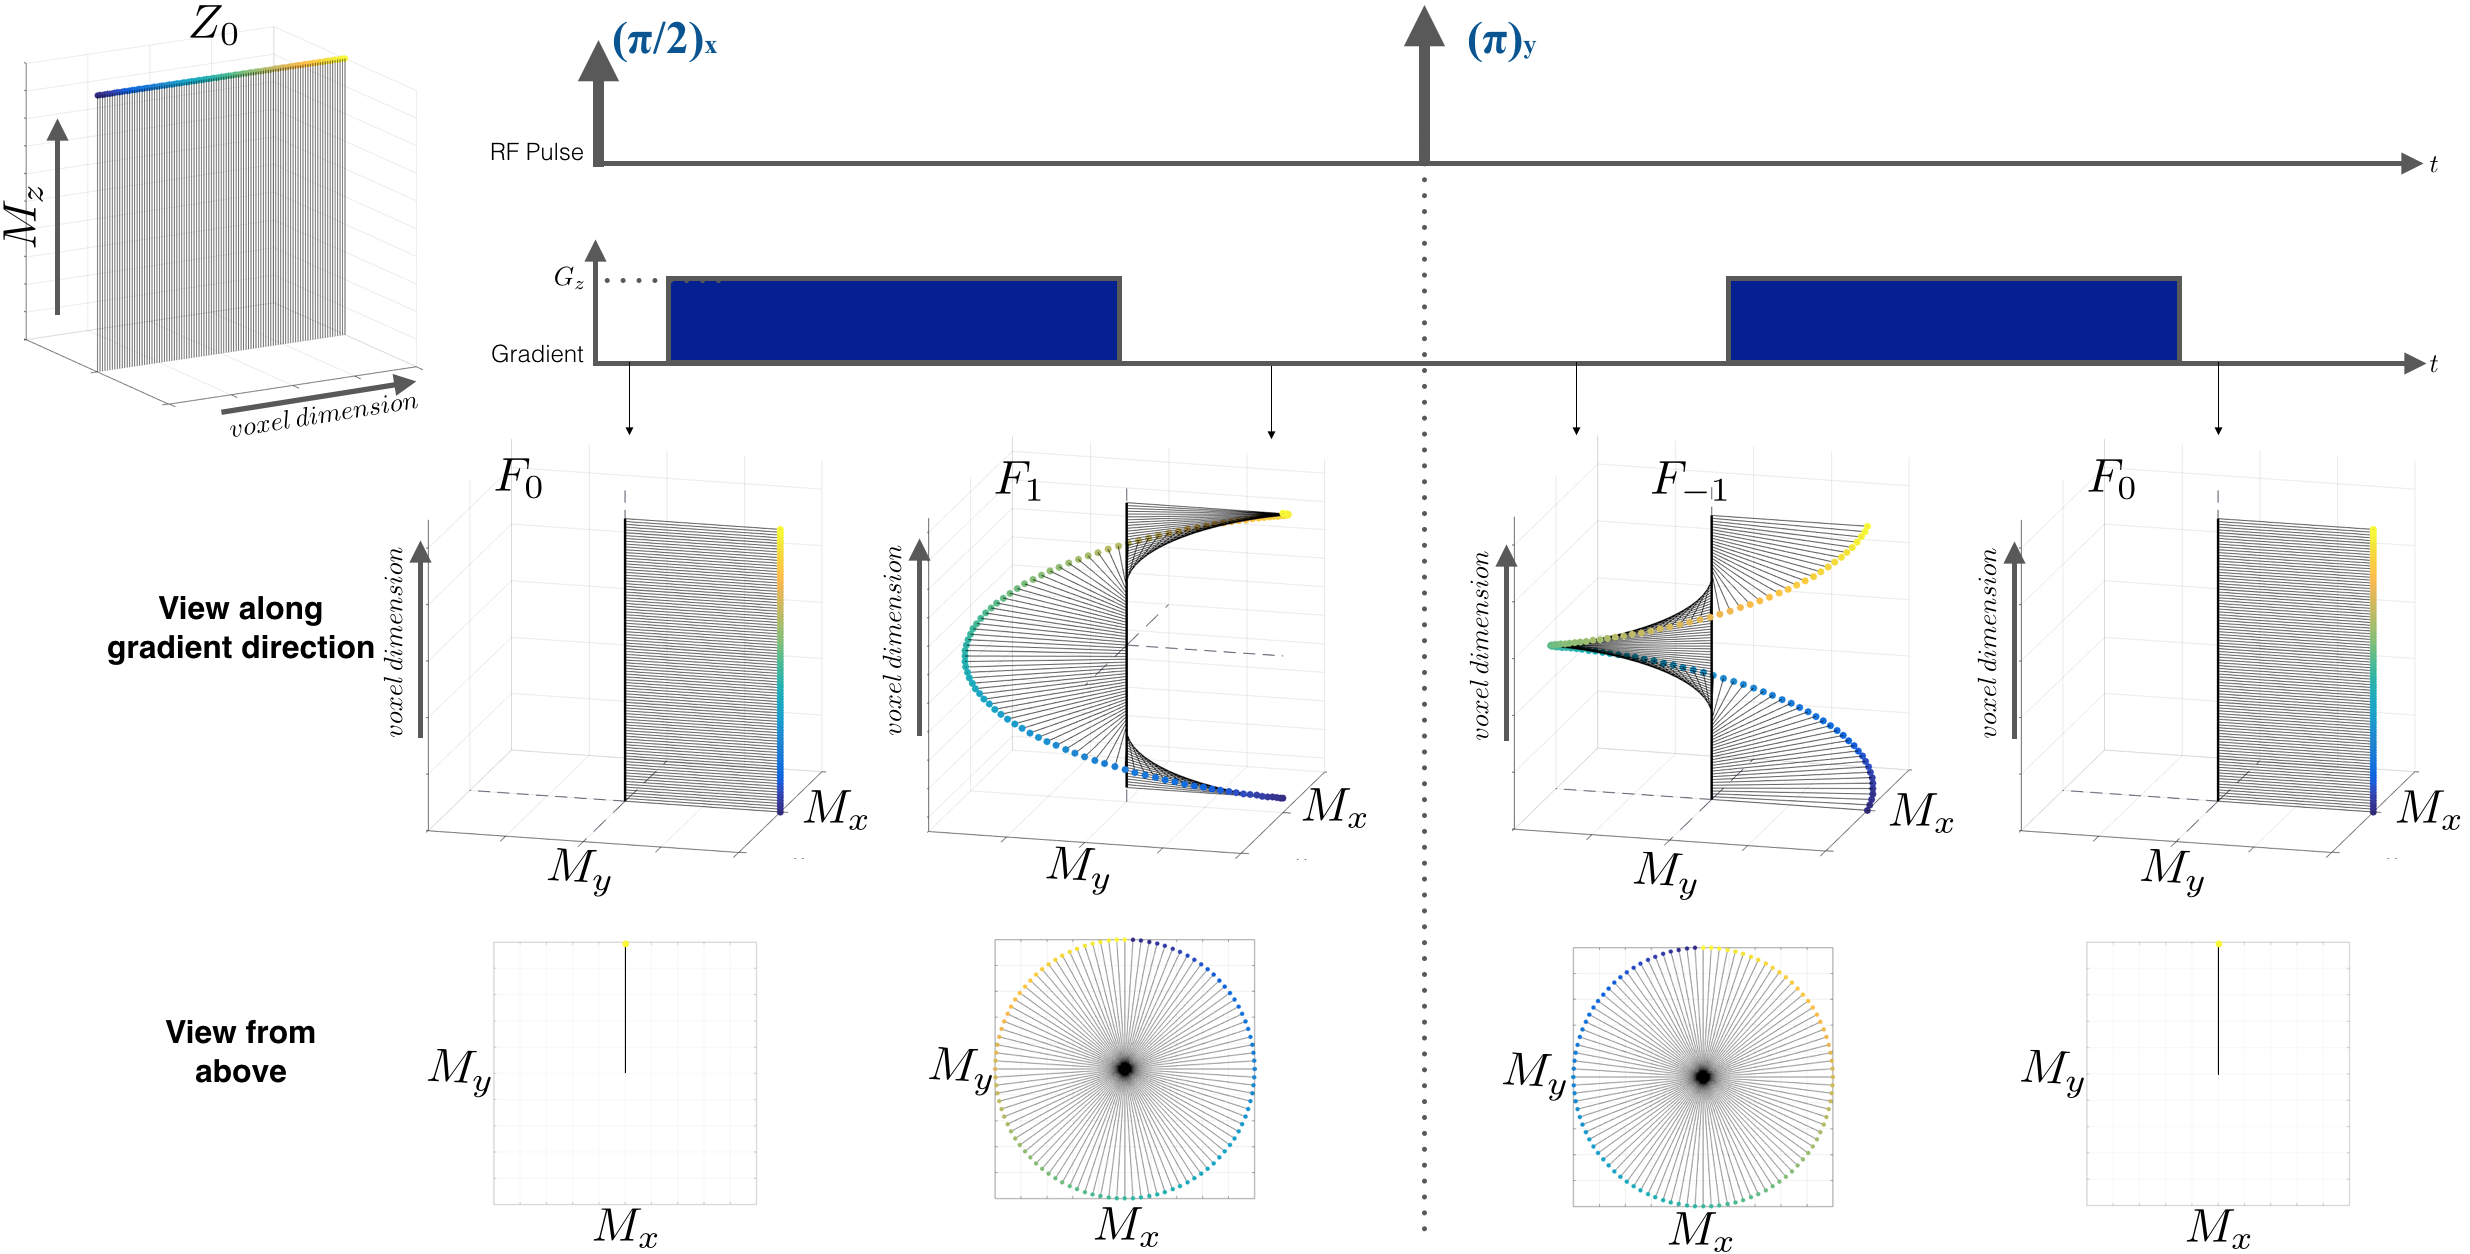
\includegraphics[angle=90,width=0.6\textwidth, keepaspectratio]{images/mrf/spinechoinepg}
    \caption{Pictorial representation of the formation of a spin echo.
    The first RF pulse flips the distribution of isochromats into the $\bm{F_0}$ configuration.
    The application of the gradient dephases the spins until the $\bm{F_1}$ configuration is formed.
    The application of the second RF pulse of flip angle $180^o$ yields the $\bm{F_{-1}}$ configuration.
    The application of the second gradient rephases the spins until they reach the coherent state $\bm{F_0}$ and an echo is formed.}
    \label{fig:spinechoinepg}
\end{figure}

The formation of the $F_{-k}$ states is best explained through an example where an RF pulse of $\alpha = \pi$ and $\phi = \pi/2$ (rotation about the y-axis) is applied on an $\bm{F_1}$ configuration.
Introducing these values in equation \ref{eq:woessner} yields:

\begin{equation}
\begin{split}
    F_{1}^+  &= - F_{-1}^- = 0 \\
    F_{-1}^+ &= - F_{1}^-  \\
    Z_{1}^+  &= - Z_{1}^- = 0
\end{split}
\end{equation}
where the $F_{-1}^-$ and $Z_{1}^-$ were set to $0$ because they were non-existent prior to the RF pulse application.
This shows that the $F_{-1}$ configuration is now formed as a consequence of applying an $180^o$ refocusing pulse.
This is the mechanism through which spin echoes are formed and a pictorial example of this happening is shown in Figure~\ref{fig:spinechoinepg}.

\hfill

The formation of the $Z_{k}$ states is best explained through an example where the RF pulse has a flip angle $\neq \pi$.
Let there be an RF pulse of flip angle $\alpha = \pi/4$ and phase angle $\phi = 0$ applied on an $\bm{F_1}$ configuration.
Introducing these values in equation \ref{eq:woessner} yields:

\begin{equation}
\begin{split}
    F_{1}^+  &= F_{1}^- cos^2(\alpha/2) \approx 0.853 F_{1}^- \\
    F_{-1}^+ &= F_{1}^- sin^2(\alpha/2) \approx 0.147 F_{1}^-   \\
    Z_{1}^+  &= - i/2 F_{1}^- sin(\alpha)  \approx - 0.353 \, i \, F_{1}^-
\end{split}
\end{equation}
which shows that the application of the RF pulse lead to a partitioning of the isochromat ensemble into three configuration states: $\bm{F_1}$, $\bm{F_{-1}}$ and $\bm{Z_1}$ of different coefficients.
Figure~\ref{fig:RFPulseinEPG} shows a pictorial representation of the effect of applying the $(\pi/4)_x$ RF pulse on a dephased $\bm{F_1}$ configuration.

\begin{figure}[ht]
    \centering
    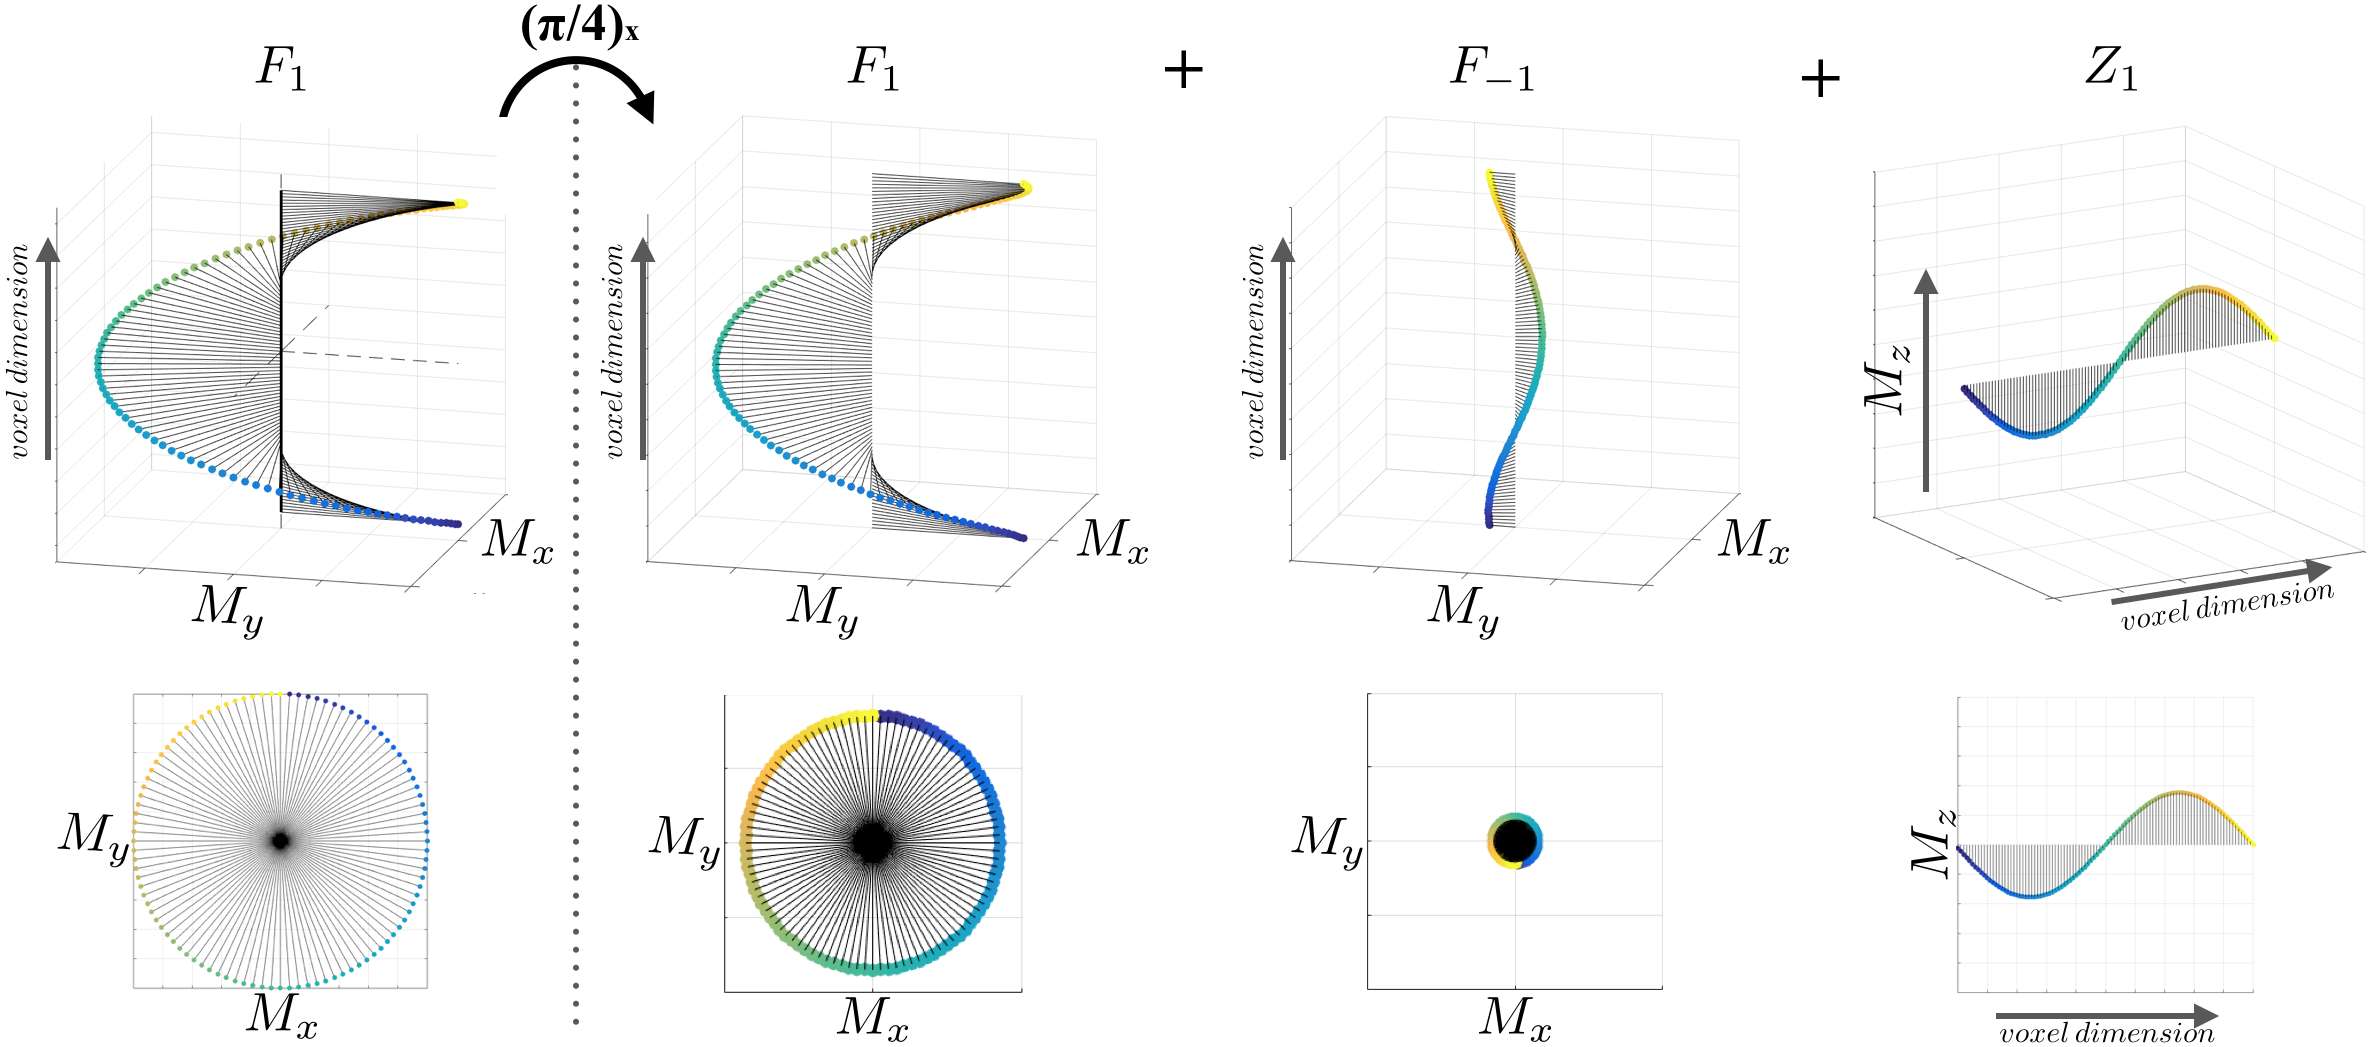
\includegraphics[angle=0,width=1\textwidth, keepaspectratio]{images/mrf/RFPulseinEPG}
    \caption{Pictorial representation of the formation of configuration states as a result of applying an RF pulse on a fully dephased $\bm{F_1}$ state.
    In this example we are showing the effect of an instantaneous RF pulse of flip angle $\alpha = \pi/4$ and phase angle $\phi = 0$ which `mixes' the populations into configuration states of the same 
    }
    \label{fig:RFPulseinEPG}
\end{figure}

\hfill

% % % % % % % % % % % % % % % % % % % % 
\textbf{Relaxation effects} 

The effects of relaxation towards thermal equilibrium can also be described in the \ac{epg} framework.
For the transverse states $T_2$ relaxation occurs: $F_k' = E_2 F_k$, while for the longitudinal states $T_1$ relaxation occurs: $Z_k' = E_1 Z_k$ (for $k \neq 0$)
%, $Z_k$ states are attenuated) 
and $Z_k' = E_1 Z_k + M_0(1 - E_1)$ (for $k = 0$).
%, $Z_k$ states experience recovery).
Here, $E_1 = e^{-\tau/T_1}$ and $E_2 = e^{-\tau/T_2}$ for a given time $\tau$.
In matrix form, this becomes \cite{Hennig1991}:

\begin{equation}\label{eq:woessnerFn}
    \begin{bmatrix}
        F_k      \\
        F_{-k} \\
        Z_k
    \end{bmatrix}' = 
    \underbrace{
    \underbrace{\begin{bmatrix}
        E_2 & 0 & 0 \\
        0 & E_2 & 0 \\
        0 & 0 & E_1 
    \end{bmatrix}
    \begin{bmatrix}
        F_k      \\
        F_{-k} \\
        Z_k
    \end{bmatrix}}_\text{for k $\neq$ 0}
    +
    \begin{bmatrix}
        0 \\
        0 \\
        M_0 (1 - E_1)
    \end{bmatrix}}_\text{for k = 0}
\end{equation}